%!TEX TS-program = xelatex
\documentclass[en]{uet-awesome-thesis} % use [vi] for vietnamese

\graphicspath{{figures/}}

\usepackage{blindtext}

\usepackage{titlesec}
\titleformat{\subsubsection}[block]{\normalfont\normalsize\bfseries}{\thesubsubsection}{1em}{}
\usepackage{microtype}

\title{HỆ THỐNG CƠ SỞ DỮ LIỆU PHÂN TÍCH DỮ LIỆU CHO WEB E-COMMERCE}
\author{Nhóm 7}
\major{Hệ quản trị cơ sở dữ liệu}
%\advisor{Prof. Lê Thanh Hà}
\university{University of Engineering and Technology}
\universitycity{Hanoi}
\degreeyear{2026}

\input{frontmatter/glossaries}
\makeglossaries 

\begin{document}

%%%%%%%%%%%%%%%%%%%%%%%%%%%%%%%%
%title 
%%%%%%%%%%%%%%%%%%%%%%%%%%%%%%%%
\maketitle
% 
%\makesidecover

%\authorship

%\approval

\authorlist{
	\begin{table}[h]
		\centering
		\begin{tabular}{|c|l|l|c|}
			\hline
			\textbf{STT} & \textbf{Họ và tên} & \textbf{MSSV} & \textbf{Vai trò} \\
			\hline
			1 & Nuyễn Bình Dương & 21020001 & Nhóm trưởng \\
			\hline
			2 & Nguyễn Văn Huy & 21020002 & Thành viên \\
			\hline
			3 & Nguyễn Khánh An & 21020003 & Thành viên \\
			\hline
			4 & Nguyễn Hai Bảy & 21020004 & Thành viên \\
			\hline
			5 & Nguyễn Minh Đức    & 21020003 & Thành viên \\
			\hline
			6 & Lò Trí Dũng   & 21020004 & Thành viên \\
			\hline
		\end{tabular}
	\end{table}
}
\pagenumbering{roman}

\addcontentsline{toc}{chapter}{Tóm tắt}
\input{frontmatter/abstract}

\tableofcontents
\addcontentsline{toc}{chapter}{Danh mục hình vẽ}
\listoffigures
\addcontentsline{toc}{chapter}{Danh mục bảng biểu}
\listoftables

\glsaddall
\printglossary[type=\acronymtype,title=Danh mục các viết tắt, toctitle=Danh mục các viết tắt]
\printglossary[type=notation,title=Danh mục ký hiệu, toctitle=Danh mục ký hiệu,nonumberlist]

\input{frontmatter/opening}

\newpage
\pagenumbering{arabic}


\begin{savequote}[75mm] 
Một hệ thống cơ sở dữ liệu tốt là nền tảng cho sức mạnh kinh doanh.
\qauthor{Dữ liệu là tài sản} 
\end{savequote}

\chapter{Giới thiệu}

\newthought{Hệ thống cơ sở dữ liệu} là một phần quan trọng trong các ứng dụng e-commerce hiện đại. Hệ thống này cho phép lưu trữ, quản lý và truy vấn lượng lớn dữ liệu một cách hiệu quả. Một thiết kế cơ sở dữ liệu tốt sẽ cải thiện hiệu suất của hệ thống, giảm chi phí vận hành và nâng cao trải nghiệm người dùng.
$$\zeta = \frac{1039}{\pi}$$


For an example of a full page figure, see Fig.~\ref{fig:myFullPageFigure}.

\section{This is section one}

\blindtext


\blindtext


\begin{figure}  
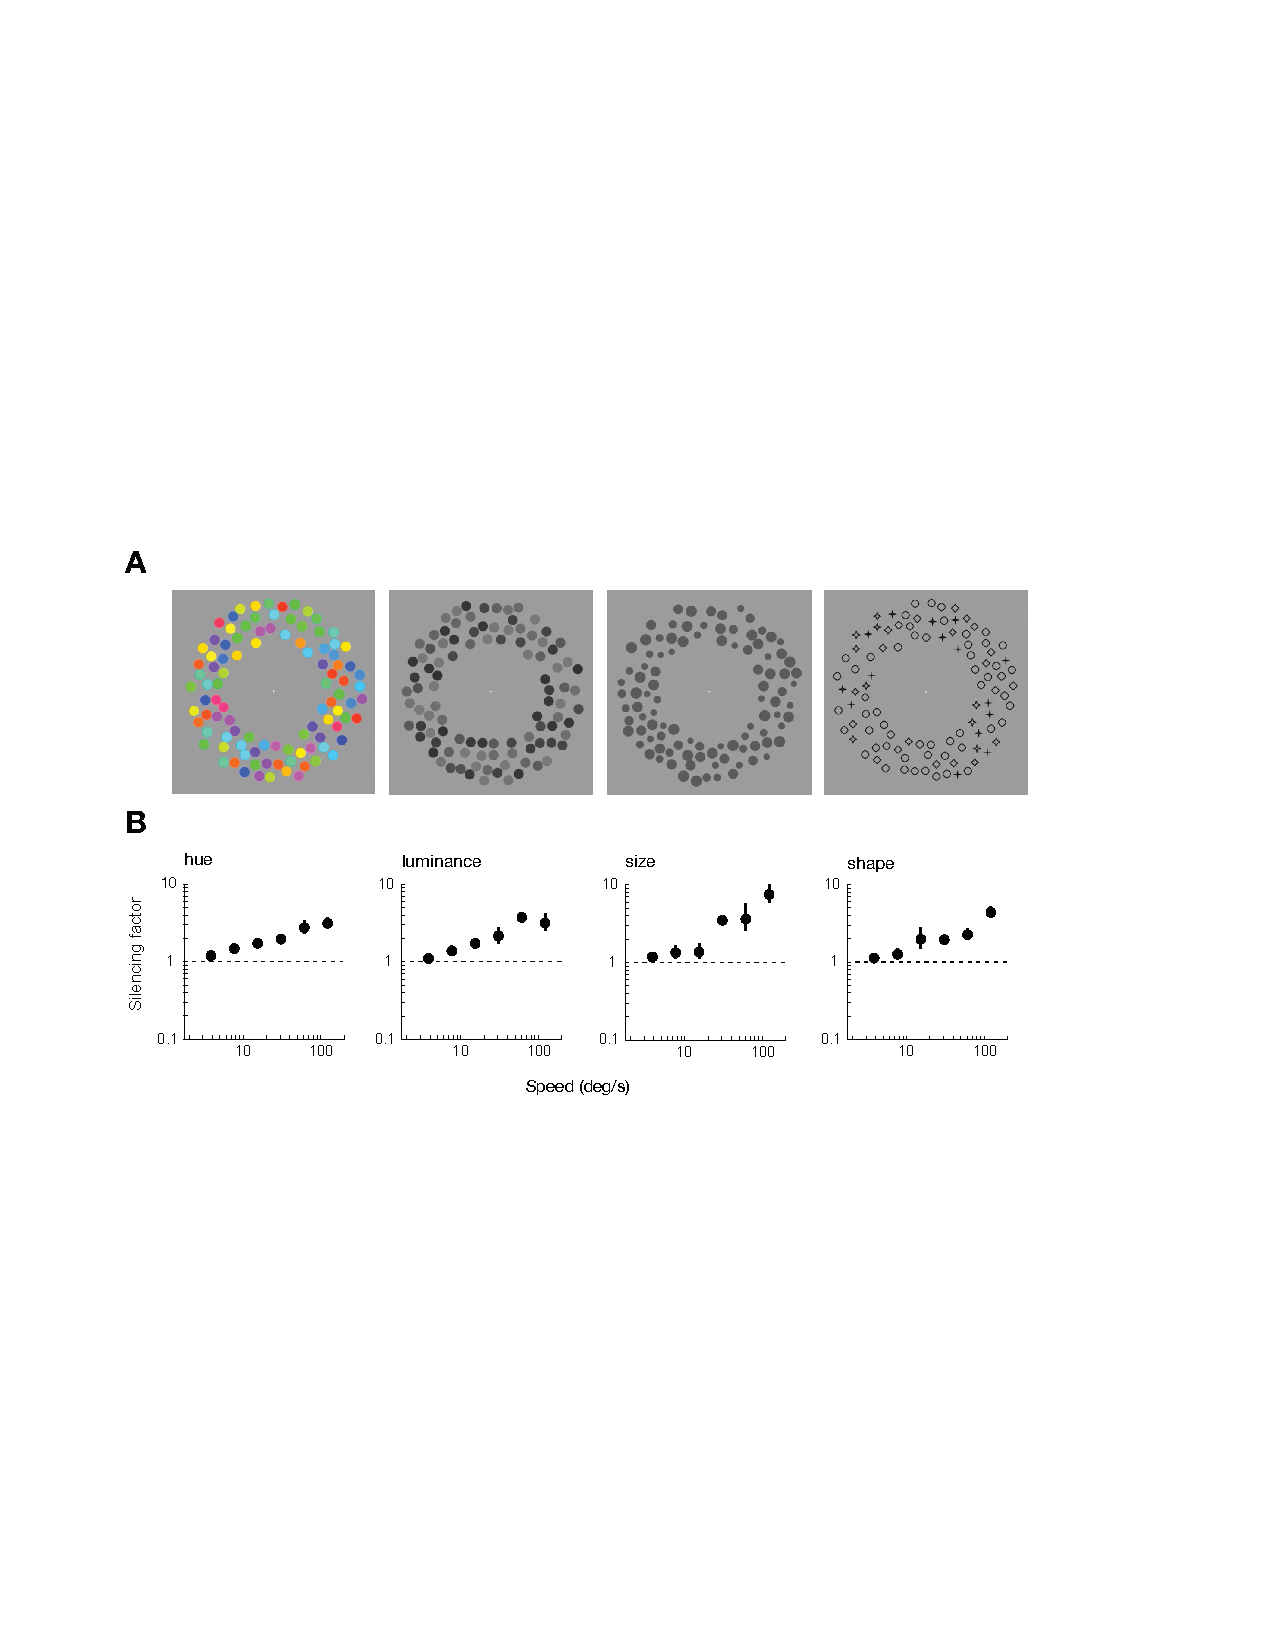
\includegraphics[width=\textwidth]{figures/fig1}
\caption[Short figure name.]{This is a figure that floats inline and here is its caption.
\label{fig:myInlineFigure}}
\end{figure}

\blindtext

\begin{figure}  
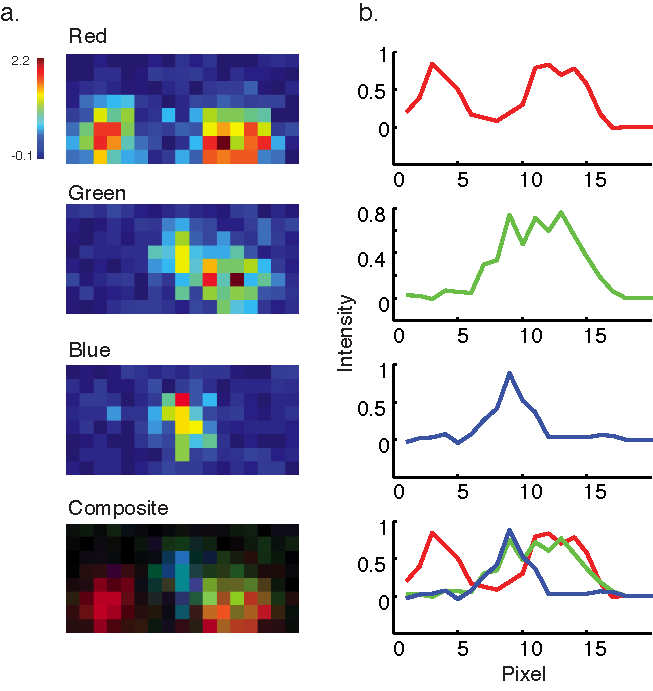
\includegraphics[width=\textwidth]{figures/fullpage}
\caption[Short figure name.]{This is a full page figure using the FPfigure command. It takes up the whole page and the caption appears on the preceding page. Its useful for large figures. Harvard's rules about full page figures are tricky, but you don't have to worry about it because we took care of it for you. For example, the full figure is supposed to have a title in the same style as the caption but without the actual caption. The caption is supposed to appear alone on the preceding page with no other text. You do't have to worry about any of that. We have modified the fltpage package to make it work. This is a lengthy caption and it clearly would not fit on the same page as the figure. Note that you should only use the FPfigure command in instances where the figure really is too large. If the figure is small enough to fit by the caption than it does not produce the desired effect. Good luck with your thesis. I have to keep writing this to make the caption really long. LaTex is a lot of fun. You will enjoy working with it. Good luck on your post doctoral life! I am looking forward to mine. \label{fig:myFullPageFigure}}
\end{figure}
\afterpage{\clearpage}

\blindtext

\section{This is section two}
\blindtext
\blindmathpaper

\section{This is section three}
\blindtext
\blindmathpaper
\begin{savequote}[75mm] 
Chức năng là yêu cầu đầu tiên để một hệ thống hoạt động hiệu quả.
\qauthor{Thiết kế hệ thống} 
\end{savequote}

\chapter{Chức năng}

\newthought{Hệ thống quản lý cơ sở dữ liệu} e-commerce cần cung cấp các chức năng cơ bản và nâng cao để hỗ trợ hoạt động kinh doanh. Các chức năng này được thiết kế dựa trên yêu cầu nghiệp vụ và đặc điểm của thị trường e-commerce.

\section{Chức năng quản lý sản phẩm}

Quản lý thông tin sản phẩm bao gồm thêm, sửa, xóa và tìm kiếm sản phẩm.

\section{Chức năng quản lý đơn hàng}

Quản lý chu trình đơn hàng từ tạo đến hoàn thành.

\section{Chức năng quản lý khách hàng}

Quản lý thông tin khách hàng, lịch sử mua hàng và ưu tiên.

\section{Chức năng báo cáo và phân tích}

Tạo báo cáo và phân tích dữ liệu bán hàng.

\section{This is section one}
\blindtext

\blinditemize

\begin{table}[tb]
  \centering
  \caption{Network constants of the energy model.}
  \label{tab:network_constants}
  \small
  % \begin{tabular*}{\textwidth}{l @{\extracolsep{\fill}} l}
  \begin{tabular}{lll}
    \toprule
    Parameter & Value & Unit \\
    \midrule
    $\epsilon_{elec}$ & $50$ &  $nJ/bit$ \\
    $\epsilon_{fs}$ & $10$ & $pJ/bit/m^2$ \\
    $\epsilon_{mp}$ & $0.0013$ & $pJ/bit/m^4$ \\
    \bottomrule
  \end{tabular}
  % \end{tabular*}
\end{table} 


\blindmathpaper

\blindtext@formula 

\section{This is section two}
\blindtext
\blindmathpaper

\section{This is section three}
\blindtext
\blindmathpaper
\chapter{Triển khai cài đặt cơ sở dữ liệu}

\newthought{Triển khai cài đặt cơ sở dữ liệu} là giai đoạn chuyển đổi lược đồ thiết kế thành các bảng, index, view và trigger thực tế. Phần này trình bày chi tiết cấu trúc từng bảng, các ràng buộc, index tối ưu hóa, view để lấy dữ liệu và trigger tự động.

\section{Account}

\subsection{Cấu trúc bảng}

Bảng \texttt{accounts} lưu trữ thông tin tài khoản hệ thống.

\begin{verbatim}
CREATE TABLE accounts (
    account_id INT PRIMARY KEY AUTO_INCREMENT,
    email VARCHAR(255) UNIQUE NOT NULL,
    password_hash VARCHAR(255) NOT NULL,
    role ENUM('buyer', 'seller', 'admin') NOT NULL,
    status ENUM('active', 'suspended', 'deleted') DEFAULT 'active',
    created_at TIMESTAMP DEFAULT CURRENT_TIMESTAMP,
    updated_at TIMESTAMP DEFAULT CURRENT_TIMESTAMP 
        ON UPDATE CURRENT_TIMESTAMP
);
\end{verbatim}

\subsection{Index}

\begin{verbatim}
CREATE INDEX idx_accounts_email ON accounts(email);
CREATE INDEX idx_accounts_role ON accounts(role);
CREATE INDEX idx_accounts_status ON accounts(status);
\end{verbatim}

\subsection{View}

\begin{verbatim}
CREATE VIEW vw_active_accounts AS
SELECT account_id, email, role, created_at
FROM accounts
WHERE status = 'active';
\end{verbatim}

\subsection{Trigger}

\begin{verbatim}
DELIMITER $$
CREATE TRIGGER trg_account_audit
AFTER UPDATE ON accounts
FOR EACH ROW
BEGIN
    INSERT INTO account_audit_log 
    (account_id, old_status, new_status, changed_at)
    VALUES (NEW.account_id, OLD.status, NEW.status, NOW());
END$$
DELIMITER ;
\end{verbatim}

\section{User}

\subsection{Table users}

Bảng \texttt{users} lưu trữ thông tin chi tiết của người dùng.

\subsubsection{Cấu trúc bảng}

\begin{verbatim}
CREATE TABLE users (
    user_id INT PRIMARY KEY AUTO_INCREMENT,
    account_id INT NOT NULL UNIQUE,
    first_name VARCHAR(100) NOT NULL,
    last_name VARCHAR(100) NOT NULL,
    date_of_birth DATE,
    gender ENUM('male', 'female', 'other'),
    avatar_url VARCHAR(500),
    bio TEXT,
    total_spending DECIMAL(15, 2) DEFAULT 0,
    created_at TIMESTAMP DEFAULT CURRENT_TIMESTAMP,
    FOREIGN KEY (account_id) REFERENCES accounts(account_id)
        ON DELETE CASCADE
);
\end{verbatim}

\subsubsection{Index}

\begin{verbatim}
CREATE INDEX idx_users_account_id ON users(account_id);
CREATE INDEX idx_users_full_name ON users(last_name, first_name);
CREATE INDEX idx_users_total_spending ON users(total_spending DESC);
\end{verbatim}

\subsubsection{View}

\begin{verbatim}
CREATE VIEW vw_user_profile AS
SELECT 
    u.user_id, u.account_id, 
    CONCAT(u.first_name, ' ', u.last_name) as full_name,
    a.email, u.total_spending, u.created_at
FROM users u
JOIN accounts a ON u.account_id = a.account_id;
\end{verbatim}

\subsubsection{Trigger}

Không có trigger riêng cho bảng users.

\subsection{Table addresses}

Bảng \texttt{user\_addresses} lưu trữ các địa chỉ của người dùng.

\subsubsection{Cấu trúc bảng}

\subsubsection{Index}

\subsubsection{View}

\subsubsection{Trigger}

\subsection{Table phone\_numbers}

Bảng \texttt{user\_phone\_numbers} lưu trữ các số điện thoại của người dùng.

\subsubsection{Cấu trúc bảng}

\subsubsection{Index}

\subsubsection{View}

\subsubsection{Trigger}

\section{Product}

\subsection{Table product}

\subsubsection{Cấu trúc bảng}

\subsubsection{Index}

\subsection{Table type}

\subsubsection{Cấu trúc bảng}

\subsubsection{Index}

\subsection{Table type\_values}

\subsubsection{Cấu trúc bảng}

\subsubsection{Index}

\subsection{Table variants}

\subsubsection{Cấu trúc bảng}

\subsubsection{Index}

\subsection{Table variant\_values}

\subsubsection{Cấu trúc bảng}

\subsubsection{Index}

\subsection{Table product\_extra\_images}

\subsubsection{Cấu trúc bảng}

\subsubsection{Index}

\subsection{Table product\_reviews}

\subsubsection{Cấu trúc bảng}

\subsubsection{Index}

\subsection{Table product\_review\_images}

\subsubsection{Cấu trúc bảng}

\subsubsection{Index}

\section{Category}

Bảng \texttt{categories} lưu trữ các danh mục sản phẩm.

\subsection{Cấu trúc bảng}

\subsection{Index}

\subsection{View}

\section{Order}

\subsection{Table orders}

\subsubsection{Cấu trúc bảng}

\subsubsection{Index}

\subsubsection{View}

\subsubsection{Trigger}

\subsection{Table order\_tracking\_locations}

\subsubsection{Cấu trúc bảng}

\subsubsection{Index}

\section{Notification}

Bảng \texttt{notifications} lưu trữ các thông báo gửi đến người dùng trong hệ thống.

\subsection{Cấu trúc bảng}

\subsection{Index}

\subsection{View}

\begin{verbatim}
CREATE OR REPLACE VIEW user_notifications_view AS
SELECT
    id,
    user_id,
    title,
    type,
    content,
    image,
    target_id,
    is_read,
    read_at,
    created_at
FROM notifications
WHERE deleted = 0
ORDER BY created_at DESC;
\end{verbatim}

\begin{verbatim}
CREATE OR REPLACE VIEW notification_unread_badge_view AS
SELECT
    user_id,
    COUNT(id) AS unread_count
FROM notifications
WHERE deleted = 0
  AND is_read = 0
GROUP BY user_id;
\end{verbatim}

\subsection{Trigger}

\begin{verbatim}
DELIMITER $$
CREATE TRIGGER trg_notifications_before_insert
BEFORE INSERT ON notifications
FOR EACH ROW
BEGIN
    IF NEW.id IS NULL OR NEW.id = '' THEN
        SET NEW.id = UUID();
    END IF;
    IF NEW.created_at IS NULL THEN
        SET NEW.created_at = NOW(6);
    END IF;
    SET NEW.is_read = 0;
    SET NEW.read_at  = NULL;
END$$
DELIMITER ;
\end{verbatim}

\begin{verbatim}
DELIMITER $$
CREATE TRIGGER trg_notifications_before_update
BEFORE UPDATE ON notifications
FOR EACH ROW
BEGIN
    IF OLD.is_read = 0 AND NEW.is_read = 1 THEN
        SET NEW.read_at = NOW(6);
    END IF;
END$$
DELIMITER ;
\end{verbatim}

\section{Shopping Cart}

Bảng \texttt{shopping\_carts} và \texttt{shopping\_cart\_items} lưu trữ thông tin giỏ hàng của người dùng.

\subsection{Table shopping\_carts}

\subsubsection{Cấu trúc bảng}

\subsubsection{Index}

\subsubsection{View}

\begin{verbatim}
CREATE OR REPLACE VIEW cart_details_view AS
SELECT
    sci.id                          AS item_id,
    sc.client_id,
    sci.variant_id,
    sci.quantity,
    sci.price_each,
    (sci.quantity * sci.price_each) AS item_total_price,
    v.thumbnail,
    p.name                          AS product_name
FROM       shopping_cart_items sci
JOIN       shopping_carts sc ON sci.shopping_cart_id = sc.id
JOIN       variants        v  ON sci.variant_id       = v.id
JOIN       products        p  ON v.product_id         = p.id
WHERE      sci.deleted = 0
  AND      sc.deleted  = 0;
\end{verbatim}

\begin{verbatim}
CREATE OR REPLACE VIEW cart_header_summary_view AS
SELECT
    client_id,
    id          AS shopping_cart_id,
    total_quantity,
    total_price AS total_cart_value
FROM shopping_carts
WHERE deleted = 0;
\end{verbatim}

\subsubsection{Trigger}

\begin{verbatim}
DELIMITER $$
CREATE TRIGGER trg_shopping_carts_before_insert
BEFORE INSERT ON shopping_carts
FOR EACH ROW
BEGIN
    IF NEW.id IS NULL OR NEW.id = '' THEN
        SET NEW.id = UUID();
    END IF;
    IF NEW.created_at IS NULL THEN
        SET NEW.created_at = NOW(6);
    END IF;
    SET NEW.total_price    = 0;
    SET NEW.total_quantity = 0;
END$$
DELIMITER ;
\end{verbatim}

\subsection{Table shopping\_cart\_items}

\subsubsection{Cấu trúc bảng}

\subsubsection{Index}

\subsubsection{View}

\subsubsection{Trigger}

\begin{verbatim}
DELIMITER $$
CREATE TRIGGER trg_shopping_cart_items_before_insert
BEFORE INSERT ON shopping_cart_items
FOR EACH ROW
BEGIN
    IF NEW.id IS NULL OR NEW.id = '' THEN
        SET NEW.id = UUID();
    END IF;
    IF NEW.created_at IS NULL THEN
        SET NEW.created_at = NOW(6);
    END IF;
END$$
DELIMITER ;
\end{verbatim}

\section{Transaction}

Bảng \texttt{transactions} lưu trữ thông tin giao dịch thanh toán.

\subsection{Cấu trúc bảng}

\subsection{Index}

\subsection{View}

\subsection{Trigger}
\begin{savequote}[75mm]
Chức năng là linh hồn của hệ thống.
\qauthor{Phát triển phần mềm}
\end{savequote}

\chapter{Triển khai các chức năng bổ sung cho hệ thống}

\newthought{Các chức năng bổ sung} đóng vai trò quan trọng trong việc nâng cao trải nghiệm người dùng và hỗ trợ quyết định kinh doanh. Phần này trình bày chi tiết cài đặt từng tính năng bao gồm giải thích cơ chế, cài đặt vật lý và câu lệnh truy vấn.

\section{Chức năng cho guest (chưa đăng nhập)}

\subsection{4.1.1 Đăng ký}

\subsubsection{Giải thích cơ chế}

Chức năng đăng ký cho phép người dùng tạo tài khoản mới. Hệ thống sẽ:
\begin{enumerate}
    \item Kiểm tra email đã tồn tại chưa
    \item Hash mật khẩu trước khi lưu
    \item Tạo bản ghi trong bảng \texttt{accounts}
    \item Gửi email xác nhận
\end{enumerate}

\subsubsection{Cài đặt vật lý}

\begin{verbatim}
CREATE TABLE registration_log (
    registration_id INT PRIMARY KEY AUTO_INCREMENT,
    email VARCHAR(255),
    registration_date TIMESTAMP DEFAULT CURRENT_TIMESTAMP,
    status ENUM('pending', 'verified', 'failed')
);

CREATE TRIGGER trg_log_new_registration
AFTER INSERT ON accounts
FOR EACH ROW
BEGIN
    INSERT INTO registration_log (email, status)
    VALUES (NEW.email, 'pending');
END;
\end{verbatim}

\subsubsection{Câu lệnh truy vấn}

\begin{verbatim}
-- Kiểm tra email tồn tại
SELECT account_id FROM accounts WHERE email = ?;

-- Thêm tài khoản mới
INSERT INTO accounts (email, password_hash, role, status)
VALUES (?, SHA2(?, 256), 'buyer', 'active');

-- Kiểm tra đăng ký mới nhất
SELECT * FROM accounts 
WHERE created_at >= DATE_SUB(NOW(), INTERVAL 24 HOUR)
ORDER BY created_at DESC;
\end{verbatim}

\subsection{4.1.2 Đăng nhập}

\subsubsection{Giải thích cơ chế}

\subsubsection{Cài đặt vật lý}

\subsubsection{Câu lệnh truy vấn}

\subsection{4.1.3 Đăng xuất}

\subsubsection{Giải thích cơ chế}

\subsubsection{Cài đặt vật lý}

\subsubsection{Câu lệnh truy vấn}

\subsection{4.1.4 Hiển thị danh mục được tìm kiếm nhiều}

\subsubsection{Giải thích cơ chế}

\subsubsection{Cài đặt vật lý}

\subsubsection{Câu lệnh truy vấn}

\subsection{4.1.5 Hiển thị sản phẩm bán chạy}

\subsubsection{Giải thích cơ chế}

\subsubsection{Cài đặt vật lý}

\subsubsection{Câu lệnh truy vấn}

\subsection{4.1.6 Hiển thị sản phẩm xem nhiều nhất}

\subsubsection{Giải thích cơ chế}

\subsubsection{Cài đặt vật lý}

\subsubsection{Câu lệnh truy vấn}

\subsection{4.1.7 Lọc sản phẩm đa tiêu chí}

\subsubsection{Giải thích cơ chế}

\subsubsection{Cài đặt vật lý}

\subsubsection{Câu lệnh truy vấn}

\section{Chức năng cho Khách hàng (Người mua) - Section 4.2}

\subsection{4.2.1 Xem tổng chi tiêu cá nhân}

\subsubsection{Giải thích cơ chế}

\subsubsection{Cài đặt vật lý}

\subsubsection{Câu lệnh truy vấn}

\subsection{4.2.2 Hiển thị lịch sử giao dịch}

\subsubsection{Giải thích cơ chế}

\subsubsection{Cài đặt vật lý}

\subsubsection{Câu lệnh truy vấn}

\section{Chức năng cho Người bán (Seller) - Section 4.3}

\subsection{4.3.1 Hiển thị sản phẩm bán chạy của shop}

\subsubsection{Giải thích cơ chế}

\subsubsection{Cài đặt vật lý}

\subsubsection{Câu lệnh truy vấn}

\subsection{4.3.2 Hiển thị sản phẩm có tỉ suất mua cao}

\subsubsection{Giải thích cơ chế}

\subsubsection{Cài đặt vật lý}

\subsubsection{Câu lệnh truy vấn}

\subsection{4.3.3 Tỉ lệ hủy/ hoàn hàng}

\subsubsection{Giải thích cơ chế}

\subsubsection{Cài đặt vật lý}

\subsubsection{Câu lệnh truy vấn}

\subsection{4.3.4 Gợi ý nhập kho}

\subsubsection{Giải thích cơ chế}

\subsubsection{Cài đặt vật lý}

\subsubsection{Câu lệnh truy vấn}

\subsection{4.3.5 Dự báo cạn kho}

\subsubsection{Giải thích cơ chế}

\subsubsection{Cài đặt vật lý}

\subsubsection{Câu lệnh truy vấn}

\subsection{4.3.6 Tăng trưởng của sản phẩm}

\subsubsection{Giải thích cơ chế}

\subsubsection{Cài đặt vật lý}

\subsubsection{Câu lệnh truy vấn}

\subsection{4.3.7 Biểu đồ doanh thu theo ngày}

\subsubsection{Giải thích cơ chế}

\subsubsection{Cài đặt vật lý}

\subsubsection{Câu lệnh truy vấn}

\subsection{4.3.8 Hiển thị danh mục bán chạy của shop}

\subsubsection{Giải thích cơ chế}

\subsubsection{Cài đặt vật lý}

\subsubsection{Câu lệnh truy vấn}

\subsection{4.3.9 Hiển thị danh mục được xem nhiều}

\subsubsection{Giải thích cơ chế}

\subsubsection{Cài đặt vật lý}

\subsubsection{Câu lệnh truy vấn}

\subsection{4.3.10 Hiển thị sản phẩm được xem nhiều}

\subsubsection{Giải thích cơ chế}

\subsubsection{Cài đặt vật lý}

\subsubsection{Câu lệnh truy vấn}

\subsection{4.3.11 Hiển thị phân bố doanh thu của sub-category}

\subsubsection{Giải thích cơ chế}

\subsubsection{Cài đặt vật lý}

\subsubsection{Câu lệnh truy vấn}

\section{Chức năng cho Admin (Quản trị viên) - Section 4.5}

\subsection{4.5.1 Hiển thị người dùng có hành vi xấu}

\subsubsection{Giải thích cơ chế}

\subsubsection{Cài đặt vật lý}

\subsubsection{Câu lệnh truy vấn}

\subsection{4.5.2 Hiển thị doanh thu của toàn sàn}

\subsubsection{Giải thích cơ chế}

\subsubsection{Cài đặt vật lý}

\subsubsection{Câu lệnh truy vấn}


\singlespacing

\clearpage
\bibliography{refs}
\addcontentsline{toc}{chapter}{References}
\bibliographystyle{plainnat}

\begin{appendices}
\chapter{Conclusion}

\section{Điểm mạnh}

Hệ thống cơ sở dữ liệu được thiết kế với các điểm mạnh sau:
\begin{itemize}
  \item Hiệu suất cao và khả năng mở rộng
  \item Bảo mật dữ liệu toàn diện
  \item Dễ dàng quản lý và bảo trì
\end{itemize}

\section{Điểm yếu}

Các hạn chế của hệ thống hiện tại:
\begin{itemize}
  \item Cần tối ưu hóa thêm cho các truy vấn phức tạp
  \item Yêu cầu quản trị viên chuyên biệt
\end{itemize}

\section{Kết luận Cuối}

Hệ thống cơ sở dữ liệu này cung cấp một nền tảng vững chắc cho ứng dụng e-commerce, hỗ trợ các chức năng kinh doanh cơ bản và nâng cao. Với sự hoàn thiện thêm, nó sẽ trở thành một giải pháp toàn diện cho quản lý dữ liệu e-commerce.
\chapter{Khuyến nghị và Hướng phát triển}

Các khuyến nghị cho phát triển tương lai của hệ thống:
\begin{itemize}
  \item Tích hợp công nghệ machine learning để phân tích dữ liệu khách hàng
  \item Cải thiện hiệu suất với caching layer
  \item Triển khai các giải pháp backup và disaster recovery
  \item Mở rộng hỗ trợ cho các thị trường quốc tế
\end{itemize}
\end{appendices}

\end{document}
